%% ISAE-SUPAERO report template for research projects 
%% V1.0
%% 2016/04/14
%% by Damien Roque
%% See http://personnel.isae.fr/damien-roque


%% This template is based on bare_conf.tex
%% V1.4b
%% 2015/08/26
%% by Michael Shell

%%*************************************************************************
%% Legal Notice:
%% This code is offered as-is without any warranty either expressed or
%% implied; without even the implied warranty of MERCHANTABILITY or
%% FITNESS FOR A PARTICULAR PURPOSE! 
%% User assumes all risk.
%% In no event shall the IEEE or any contributor to this code be liable for
%% any damages or losses, including, but not limited to, incidental,
%% consequential, or any other damages, resulting from the use or misuse
%% of any information contained here.
%%
%% All comments are the opinions of their respective authors and are not
%% necessarily endorsed by the IEEE.
%%
%% This work is distributed under the LaTeX Project Public License (LPPL)
%% ( http://www.latex-project.org/ ) version 1.3, and may be freely used,
%% distributed and modified. A copy of the LPPL, version 1.3, is included
%% in the base LaTeX documentation of all distributions of LaTeX released
%% 2003/12/01 or later.
%% Retain all contribution notices and credits.
%% ** Modified files should be clearly indicated as such, including  **
%% ** renaming them and changing author support contact information. **
%%*************************************************************************

\documentclass[conference]{IEEEtran}

\usepackage[utf8]{inputenc}
\usepackage{ifthen}
\usepackage{cite}
\usepackage[pdftex]{graphicx}
\graphicspath{{images/}}
\usepackage{tikz,filecontents}
\usetikzlibrary{shapes,arrows,shadings,patterns}
\usepackage{pgfplots}
\pgfplotsset{compat=newest}
\pgfplotsset{plot coordinates/math parser=false}
\newlength\figureheight
\newlength\figurewidth

\usepackage{amsfonts}
\usepackage[cmex10]{amsmath}
\usepackage{multirow}
\usepackage{amssymb}
\usepackage{hyperref}
\usepackage{graphicx}
\usepackage{amssymb}
\usepackage{amsmath}
\usepackage{amsthm}
\usepackage{dsfont}
\usepackage{caption}
\usepackage{graphicx}
\usepackage{pgfplots}
\usepackage{tikz}

% Examples of several macros
\newcommand*{\SET}[1]{\ensuremath{\boldsymbol{#1}}}
\newcommand*{\VEC}[1]{\ensuremath{\boldsymbol{\mathrm{#1}}}}
\newcommand*{\FAM}[1]{\ensuremath{\mathrm{#1}}}
\newcommand*{\MAT}[1]{\ensuremath{\boldsymbol{\mathrm{#1}}}}
\newcommand*{\OP}[1]{\ensuremath{\mathrm{#1}}}
\newcommand*{\NORM}[1]{\ensuremath{\left\|#1\right\|}}
\newcommand*{\DPR}[2]{\ensuremath{\left \langle #1,#2 \right \rangle}}

\newtheorem{theorem}{Theorem}

\newcommand{\alert}[1]{\textcolor{red}{#1}}
\usepackage[caption=false,font=footnotesize]{subfig}
\usepackage{url}
\usepackage{amsfonts}

% correct bad hyphenation here
\hyphenation{op-tical net-works semi-conduc-tor}


\begin{document}
%
% paper title
% Titles are generally capitalized except for words such as a, an, and, as,
% at, but, by, for, in, nor, of, on, or, the, to and up, which are usually
% not capitalized unless they are the first or last word of the title.
% Linebreaks \\ can be used within to get better formatting as desired.
% Do not put math or special symbols in the title.
\title{PIR : Mixed-initiative mission}

% for over three affiliations, or if they all won't fit within the width
% of the page, use this alternative format:
% 
	\author{\IEEEauthorblockN{Vagneron Thomas\IEEEauthorrefmark{1},
Caroline Carvalho Chanel\IEEEauthorrefmark{2},Raphaelle N. Roy\IEEEauthorrefmark{2} and
Nicolas Drougard\IEEEauthorrefmark{2}}
\IEEEauthorblockA{\IEEEauthorrefmark{1}Institut Supérieur de l'Aéronautique et de l'Espace (ISAE-SUPAERO), Université de Toulouse, 31055 Toulouse, FRANCE\\
Email: \{thomas.vagneron\}@student.isae-supaero.fr}
\IEEEauthorblockA{\IEEEauthorrefmark{2}Institut Supérieur de l'Aéronautique et de l'Espace (ISAE-SUPAERO), Université de Toulouse, 31055 Toulouse, FRANCE\\
Email: \{caroline.chanel,raphaelle.roy,nicolas.drougard\}@isae-supaero.fr}

}


%\IEEEspecialpapernotice{(Bibliography report)}
\IEEEspecialpapernotice{(Final report)}


% make the title area
\maketitle

% As a general rule, do not put math, special symbols or citations
% in the abstract
\begin{abstract}
Missions involving robots are prone to be more and more present, as the use of machines and their autonomy increase rapidly.
In Mixed-Initiative missions, \textit{i.e.} missions benefiting from the skills of both a robot and a human operator,  
the latter is often thought as omniscient in the literature. 
However many examples show that human factors are involved in mission failures. 
Our project is thus to improve human-robot missions by taking into account potential weaknesses of human operators 
instead of considering them as always reliable.
For this end we propose to use Probabilistic Planning (MOMDP) and Reinforcement Learning in order to compute a strategy
meant to optimally inform the operator during the mission and allocate tasks between human and robot.
The proposed proof of concept mission concerns a human-robot team which has to extinguish fires.
This report is dedicated to the robot actions computation given to human behavior. 
Simulation environments representing the firefighter mission have been developed and agents have been trained on them.
The general project is first described to highlight the problem as well as the proposed solution and tools.
Then we introduce Reinforcement Learning and give some details about the algorithm TD($\lambda$), 
improving strategies after some simulations of any environment.
Finally the developed simulation environments are described along with the scores obtained by a TD($\lambda$) agent on it
for different parameters.
\end{abstract}


\IEEEpeerreviewmaketitle

\section{Context}
\label{sec:problem-statement}
The increasing autonomy of robots 
led to make use of them in a more 
and more large range of operations and activities,
for instance in rough places for surveillance or inspection of contaminated sites.
Because the machines cannot be held responsible in case of failure and do not
possess the human creativity to improvise, those activities require the assistance of humans. In
a mission led by an autonomous robot under the surveillance of a human operator or pilot, the
latter is often viewed as a providential agent, capable of resolving any problem and responding
to a failure of the robot instantly. But many factors can also lead to a failure of the mission,
regarding the human intervention, such as a misinterpretation of the information given to the
pilot (due to e.g. a poor designed user interface) or the tunneling of the human operator 
on a certain task or point of the mission \cite{LDARGENT2016}

%% FUNCTION ALLOCATION PART
Regarding the state of the art, the "Fitts list" \cite{FITTS}, 
which is a compilation of the general strengths and weaknesses of machines and humans, 
was traditionally used to determine the function allocation between human and machines. 
% define allocation function
The allocation function is the function that defines the actions that humans and machines are allowed to do, i.e. their role during the mission. 
In order to determine the level of human versus autonomy involvement, it is important to know the individual strengths of each actor. On the one hand, humans are capable of complex social interactions, moral judgment, operate well in dynamics environments and are highly flexible. On the other hand, the machines are capable of higher computational performance, produce repeatable results, can handle multiple tasks simultaneously and are not prone to fatigue or boredom \cite{NOTHWANG}.

%% COUNTERMEASURE PART
A problem still lies in the fact that the operator is considered as an external help, 
capable of resolving all the problems encountered by the machine. 
In fact, the human operator should no be considered like this, but as a part of a team.
% why? because of the previously mentioned issues (regarding human intervention)
Because of the previously mentioned issues : the human operator is not always reliable. He is subject to boredom, fatigue, stress and many others factors that can contribute to lessen its efficiency during the mission.
Considering this fact, the operator should be monitored to consider if he is capable of making accurate decisions, and allow the use of countermeasures (visual stimuli or alarm). 

Our idea is to use Probabilistic Planning in order to decide when the system produce countermeasures for the human-operator, and distribute the tasks between human and robot.

While we know all the information about the machine and its states, we know nothing about the states of the human operator. 
It has been shown in \cite{SOUZA} that the use of a Mixed Observability Markov Decision Process (MOMDP)
 model \cite{ONG} was relevant to compute a useful policy taking into account the partially observable cognitive state of the operator.
MOMDP are a planning framework for computing optimal sequence of actions over time. The action sequence is called policy.

The cognitive ability of the human operator can be inferred via an eye-tracker device \cite{GATEAU}, 
which shows areas where the operator focuses its attention. Also, the operator's heart beat states, observable via an electrocardiogram (ECG), 
are successful indicators of cognitive load \cite{WILSON}. 
The ECG can be coupled with an Eye-Tracker (ET) in order to detect if the operator is in a state of tunneling, and able to take accurate decisions \cite{rachelson2011optimal}. % Ref Rachelson
These data define the observations of the MOMDP.

% CONCLUSION intro
As mentionned previously, our assumption is that the human operator is not reliable.
Our goal is to optimize the mission of a human-robot team using observations from this system.
As a proof of concept, we defined a mission of type "search and fight", which consists in extinguishing fire that will spread over trees in a area with the help of a robot and a user interface.

\begin{figure}
  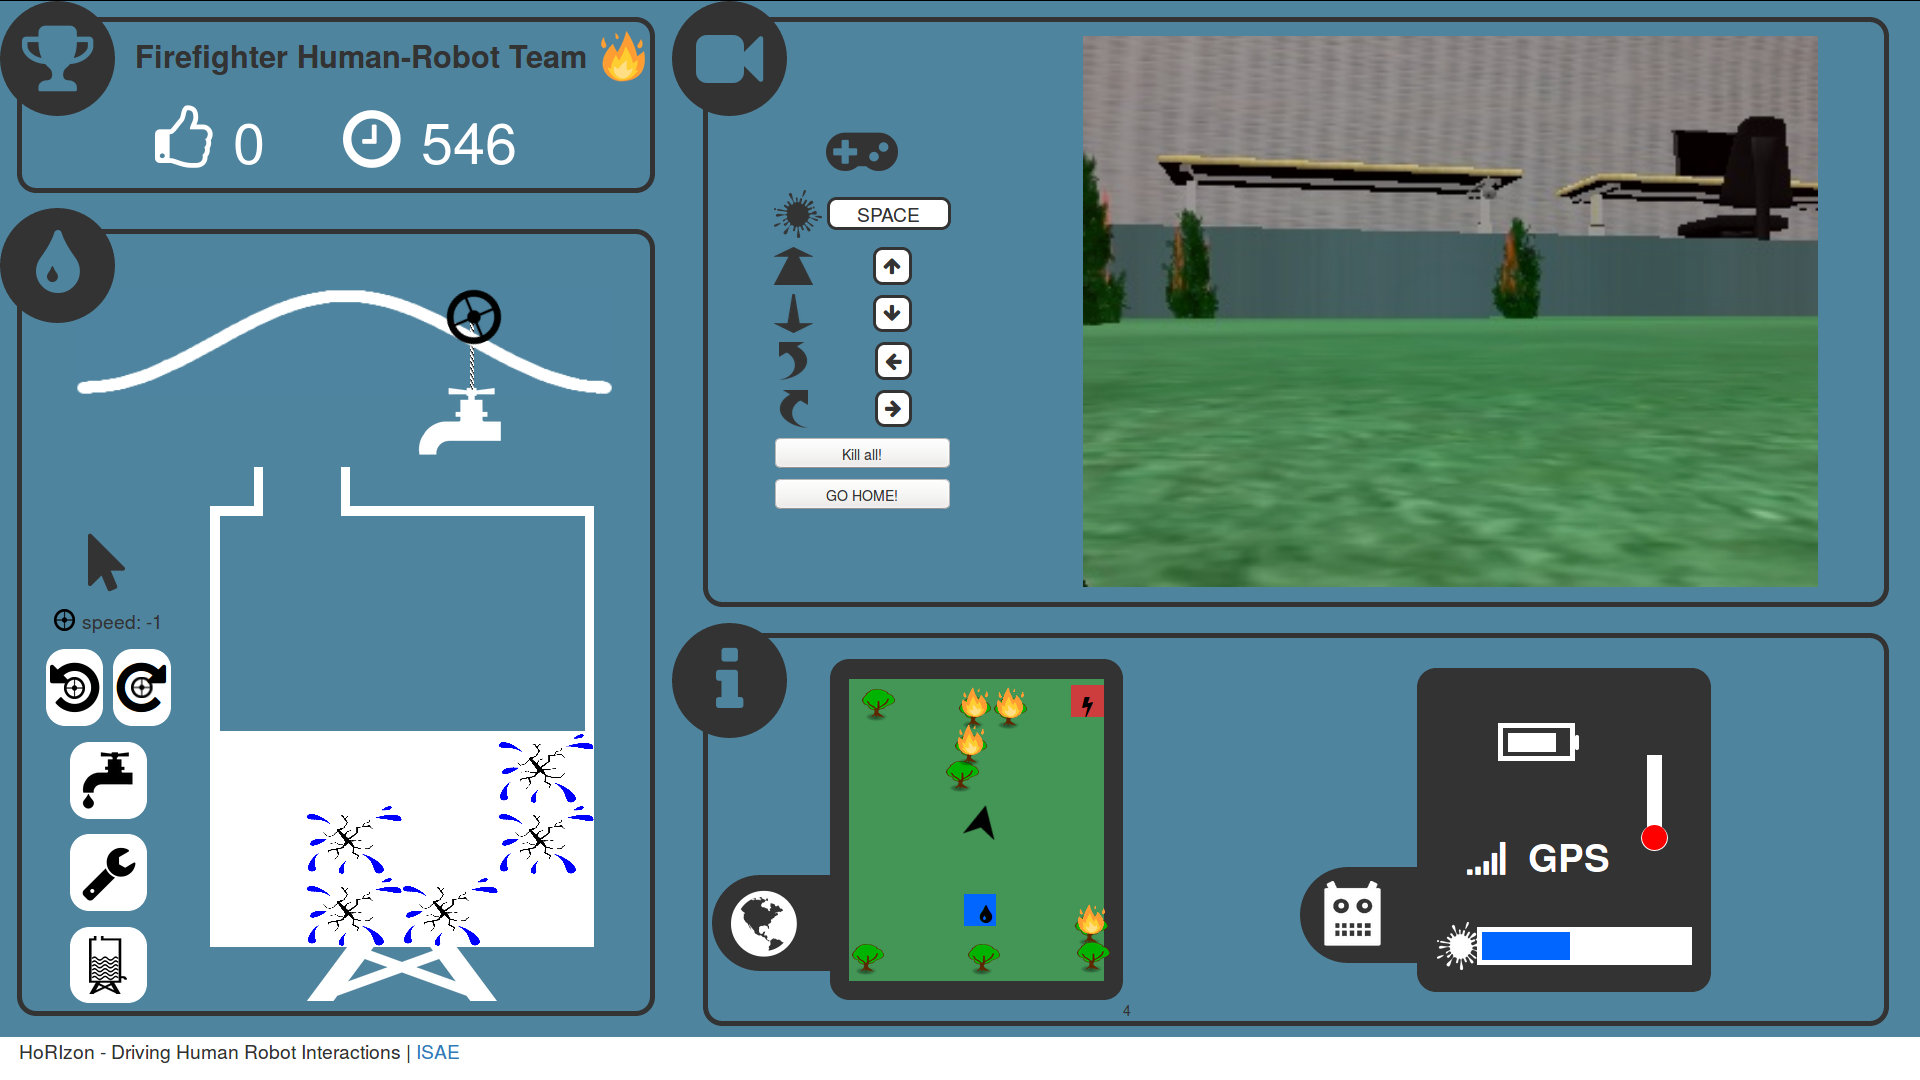
\includegraphics[scale = 0.13	]{images/Website.png}
  \caption{View of the user interface}
  \label{fig:my-figure}
\end{figure}

%(fire, battery => stress, shared tasks (navigation), clear optimization (extinguish fires),
The number of fires, the battery level or water level are stressing elements. The navigation is a shared task. The ultimate goal of the mission is the optimization of the number of extinguish fire.
The MOMDP model will be built using data from a website (i.e. the user interface) with a simulation of the environment.
The work developed in this report concerns the optimization of robot's actions given a human behavior.
We proposed to compute accurate strategies for the robot by using Reinforcement Learning (RL).

%The project presented here is a part of a bigger project that consist in the development of an operator monitoring system using an ET and an ECG, 
%because our point of view is that the human operator is not a providential agent \cite{SOUZA}, but an autonomous agent, not always reliable, of the team. 
%Our goal is to make that the ensured performance will be better when the operator is working with the robot. 
%We will develop here the development of the reinforcement learning environment (RL) which will allow us to test, improve and optimize the policy of the machine in a task of search and extinguish (it is a firefighter robot) in order to integrate the human monitoring system to harvest data to improve this system via an website (the interface is visible with the figure 1).

%\begin{figure}[htp]
%  \centering
%  \setlength\figureheight{5cm}
%  \setlength\figurewidth{6cm}
%  % This file was created by matlab2tikz.
% Minimal pgfplots version: 1.3
%
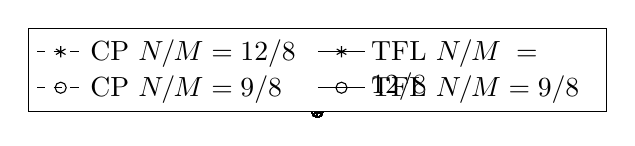
\begin{tikzpicture}

\begin{axis}[%
width=\figurewidth,
height=\figureheight,
at={(0\figurewidth,0\figureheight)},
scale only axis,
separate axis lines,
every outer x axis line/.append style={black},
every x tick label/.append style={font=\color{black}},
xmin=0,
xmax=600,
xlabel={$l_0$},
xmajorgrids,
every outer y axis line/.append style={black},
every y tick label/.append style={font=\color{black}},
ymin=15,
ymax=20,
ylabel={Gain [dB]},
ymajorgrids,
%legend style={legend cell align=left,align=left,draw=black}
legend columns=2,
legend style={text width=8em,legend cell align=left,align=left,draw=black,at={(0.5,1.05)}, anchor=south}
]
\addplot [color=black,dashed,mark=asterisk,mark options={solid}]
  table[row sep=crcr]{%
0	18.2390874094432\\
32	18.2390874094432\\
64	18.2390874094432\\
96	18.2390874094432\\
128	18.2390874094432\\
160	18.2390874094432\\
192	18.2390874094432\\
224	18.2390874094432\\
256	18.2390874094432\\
288	18.2390874094432\\
320	18.2390874094432\\
352	18.2390874094432\\
384	18.2390874094432\\
416	18.2390874094432\\
448	18.2390874094432\\
480	18.2390874094432\\
512	18.2306327719818\\
544	17.9540613758438\\
576	17.6689966399943\\
};
\addlegendentry{CP $N/M=12/8$};

\addplot [color=black,solid,mark=asterisk,mark options={solid}]
  table[row sep=crcr]{%
0	19.9999796047627\\
32	19.9782454264971\\
64	19.9172921503127\\
96	19.819523640774\\
128	19.6869764401989\\
160	19.5221481900787\\
192	19.3264690408576\\
224	19.1028168133025\\
256	18.8524145582619\\
288	18.5769651836831\\
320	18.2797229467138\\
352	17.9588025753321\\
384	17.6198925633198\\
416	17.2597387528296\\
448	16.8807108312221\\
480	16.4832729985219\\
512	16.0669779302672\\
544	15.6289248101717\\
576	15.1692321920288\\
};
\addlegendentry{TFL $N/M=12/8$};

\addplot [color=black,dashed,mark=o,mark options={solid}]
  table[row sep=crcr]{%
0	19.4884747755262\\
32	19.4884747755262\\
64	19.4884747755262\\
96	19.4884747755262\\
128	19.4800794761447\\
160	19.2039363265844\\
192	18.9194155478691\\
224	18.6243664611488\\
256	18.3193439905467\\
288	18.0035198444507\\
320	17.6753775333409\\
352	17.3329477537639\\
384	16.9775142144053\\
416	16.6049465654203\\
448	16.2214034199632\\
480	15.8132879400791\\
512	15.3931020845481\\
544	14.9429381335956\\
576	14.4724841527662\\
};
\addlegendentry{CP $N/M=9/8$};

\addplot [color=black,solid,mark=o,mark options={solid}]
  table[row sep=crcr]{%
0	19.9999188401472\\
32	19.9198402053393\\
64	19.7226565216249\\
96	19.4581952942028\\
128	19.165296513424\\
160	18.8621944283946\\
192	18.5462056497272\\
224	18.2187733804306\\
256	17.8809942229679\\
288	17.5256445475455\\
320	17.1574123511579\\
352	16.769914008492\\
384	16.3698267920046\\
416	15.9497164928657\\
448	15.5024807138218\\
480	15.0375569039195\\
512	14.5394847970002\\
544	14.0174757064722\\
576	13.4597208888491\\
};
\addlegendentry{TFL $N/M=9/8$};

\end{axis}
\end{tikzpicture}%
%  \caption{User interface (internet site/in situ) of the "firefighter team mission"}
%  \label{fig:my-figure}
%\end{figure}

\section{Theory}
\label{sec:theory}

Firstly, let us give a little bit of history about RL : the birth of RL came from the encounter in the late 70s between the computational neurosciences (reinforcement of the synaptic weights of neuronal transmission) and the experimental psychology (animal conditioning models : reinforcement of the behavior leading to satisfaction, \textit{e.g.} Pavlov's dogs experiment) 
with an adequate mathematical environment : dynamic programming.

A link with experimental psychology is the law of effects of Thorndike (1911) \cite{MUNOS1}
 : "Of several responses made to the same situation, those which are accompanied or closely followed by satisfaction to the animal will, other things being equal, be more firmly connected with the situation, so that, when it recurs, they will be more likely to recur : those which accompanied or closely followed by discomfort to the animal will, other things being equal, have their connections with that situation weakened, so that, when it recurs, they will be less likely to occur. The greater the satisfaction or discomfort, the greater the strengthening or weakening of the bond".

And so, what is Reinforcement Learning? It is an approach, here computational, to decision-making, understanding and goal-directed learning. 
The individual learns from direct contact with the environment. 
It only needs the definition of the interactions between a learning agent and its environment, in terms of states, actions and rewards.
The states represent the description of the environment.
The actions are the possible agent's actions.
Finally the rewards define the goal of the mission given to the agent.

The value and value functions are concepts that are key features of RL methods. Value functions are essential for an efficient search in the space of policies. 
The value functions are defined over the state space : \\
for $x \in X, V(x)$ is the mean of the sum of the rewards over time for a process starting in $x$.
\[ V^{\pi}(x) = \mathbb{E} [ \sum_{t \geqslant 0} r(x_t,\pi(x_t)) | x_0 = x  ] \]

Continuing on that point, the objectives of RL are : the automatized acquisition of skills for decision making in a complex and uncertain environment and learning by "experience" a behavioral strategy (named policy) reflecting the failures and success (reinforcements or rewards).

Some examples of achievements of Reinforcement learning are :\textit{cartpole} (inverted pendulum on a controlled cart), the production of the best player of backgammon, chess and more recently go (algorithm \textit{alphago}) \cite{silver2016mastering}, etc.

To begin with the theory, we need first to understand what are a Markov chain, a Markov Decision Process (MDP) and dynamic programming \cite{MUNOS1}.

A Markov chain is a dynamic system with discrete time $(x_t)_{t\in\mathbb{N}} \in X$, where $X$ is space of states such as:

\begin{equation*}
\mathbb{P}(x_{t+1}=x|x_t,x_{t-1},...,x_0)=\mathbb{P}(x_{t+1}=x|x_t).
\end{equation*}
Indeed the Markov property states that all the useful information for the future prediction is in the present state. 
A Markov chain in $X$ is defined by a initial state $x_0$ and the probability of transition $p(y|x)=\mathbb{P}(x_{t+1}=y|x_t=x)$.

Next come the MDP, which is defined by $(X,A,p,r)$, where:
\begin{itemize}
 \item $X$ space of states
 \item $A$ space of actions
 \item $p(y|x,a)$ : probability of transition from a state $x \in X$ to $y \in X$ when the action $a \in A$ is chosen:
 \begin{equation*}
 p(y|x,a) = \mathbb{P}(x_{t+1}=y|x_t=x,a_t=a),
 \end{equation*}
 \item $r(x,a,y)$ : reward when passing from $x$ to $y$ using the action $a$.
\end{itemize}
We will note here $V$ the value function and $\pi$ (with $\pi: X \rightarrow A$) the policy.\\


Dynamic programming possess two types of iterations : iterations on the values and iterations on the policies. 
In each of these algorithms a policy sequence is built,
beginning with a given initial policy $\pi_0$, and every step $k$, we evaluate the policy $\pi_k$ and calculate $V^{\pi_k}$, then we improve the policy by calculating $\pi_{k+1}$ given by $V^{\pi_k}$ :
\[ \pi_{k+1}(x) \in \mbox{arg} \mbox{max}_{a \in A}[r(x,a) + \gamma\sum_yp(y|x,a)V^{\pi_k}(y)] 	\]
We stop when $V^{\pi_k} = V^{\pi_{k+1}}$.
It's important to note that the sequence $(V^{\pi_k})_k$ is a increasing sequence. Therefore, because there is a finite number of possible policies, the termination criteria is obligatory satisfied with k. So we have $V^{\pi_k} = V^*$ where $V^*$ is the optimal value function, therefor $\pi_k$ is the optimal policy.
Some methods of solving are :
\begin{itemize}
 \item \textbf{Direct solving} of the linear system $(I-\gamma P^{\pi})V^{\pi} = r^{\pi}$. That's the Gauss elimination method, but it have a complexity of $O(N^3)$
 \item \textbf{Iteration on the values for a permanent policy} : we iterate on the operator $T^{\pi}$ (Bellman operator defined by $T^{\pi}V(x) = r(x, \pi(x))+\sum_{x'} p(x'|x,a)V(x')$). Considering a given value function $V_0$, and the recursion $V_{n+1} = T^{\pi} V_n$. 
We have then convergence of $V_n$ toward $V^{\pi}$. The problem is that the convergence is asymptotic, but the advantage is that it as a lower complexity than the direct solving method ($O(N^2 \frac{log(1/\epsilon)}{log(1/\gamma)})$ for an approximation of $\epsilon$ (interesting if $\gamma$ is not too close to 1)).
 \item \textbf{Monte-Carlo} : we simulate $n$ trajectories $((x_t^i)_{t \geqslant 0})_{1 \leqslant i \leqslant n}$, starting from $x$ and following the policy $\pi$ : $x_{t+1}^i ~ p(.|x_t^i,\pi(x^i_t))$ , so :
 \begin{equation*}
 V^{\pi}(x) \approx \frac{1}{n} \sum_{i=1}^n \sum_{t \geqslant 0} \gamma^t r(x^i_t, \pi(x^i_t)).
 \end{equation*}
 this method is interesting if we want to evaluate a unique state. It has an approximation error of order $O(1/\sqrt{n})$
 \item \textbf{Temporal differences TD($\lambda$)} : This is a smart method for using the trajectories to evaluate all the states crossed by those trajectories, by evaluating the value of a state $x$, by the sum of the observed temporal differences $r_t+\gamma V(x_{t+1}) - V(x_t)$ at the future instants t, weighted by a "trace" $\lambda$. The algorithm of TD($\lambda$) will be treated later.
\end{itemize}

During the experiments (in section III, as our work will focus on it), we used some algorithms (Cross Entropy Method (CEM), REINFORCE and TD($\lambda$)). 
We will focus here on the TD($\lambda$) method, which we found giving the most reliable results during the experiments. 
We used a random agent, i.e. selecting actions randomly, in order to test the environment.
It is important to note that the Random method was used to test the environment, and the debugging of it.
\\
\textbf{Temporal Differences TD($\lambda$)}
\\
	

\textbf{Algorithm TD($\lambda$)} \cite{sutton1988learning}: % CITER !
 After the observation of a trajectory $(x_0,x_1,...,x_K = 0)$, we update $V_n$	 to the states $(x_k)_0 \leqslant k<K$ following :

%@article{sutton1988learning,
%  title={Learning to predict by the methods of temporal differences},
%  author={Sutton, Richard S},
%  journal={Machine learning},
%  volume={3},
%  number={1},
%  pages={9--44},
%  year={1988},
%  publisher={Springer}
%}


\begin{eqnarray*}
V_{n+1}(x_k) = V_n(x_k) + \eta_n(x_k)\sum_{l=k}^{K-1}\lambda^{l-k}d_l,\\ 
\mbox{ where } d_l = r^{\pi}(x_l) + V_n(x_{l+1})-V_n(x_l).
\end{eqnarray*}

%\[ d_l = r^{\pi}(x_l) + V_n(x_{l+1})-V_n(x_l). 	\]
with $\eta_n$ the learning step, typically $\frac{1}{n}$.

The impact of the temporal differences of future transitions on the estimation of the current state value is controled by $\lambda$. TD($\lambda$) is a compromise between : 
\begin{itemize}
 \item \textbf{TD($0$)} (to estimate the fixed point of the operator of Bellman $T^{\pi}$): 
 \begin{equation*}
  V_{n+1}(x_k) = V_n(x_k) + \eta_n(x_k)d_k. 
 \end{equation*}
 \item \textbf{TD(1)} (to estimate the mean): 
 \begin{equation*} 
 V_{n+1}(x_k) = V_n(x_k) + \eta_n(x_k)\sum_{l\geqslant k}d_l. 
 \end{equation*} 
\end{itemize}

%\textbf{implementation of TD($\lambda$)} :

%With the eligibility trace $z_n \in \mathbb{R}^N$. Once the transition form $x_k$ to $x_{k+1}$ observed, we can calculate the temporal difference $d_k = r^{\pi}(x_k)+V_n(x_{x+1})-V_n(x_k)$ and update the eligibility trace :


%\begin{equation*}
% \left \{
%   \begin{split}
%    \lambda_{z_{n-1}}(x)  \text{ if } x \ne x_k \\
%    1+\lambda_{z_{n-1}}(x) \text{ if } x = x_k \\
%    0 \text{ if } x_k = 0
%   \end{split}
% \right.
%\end{equation*}

%and we iterate, for every $x$, 
%\begin{equation*}
%V_{n+1}(x) = V_n(x) + \eta_n(x)z_n(x)d_n.
%\end{equation*}

\textbf{the choice of $\lambda$} :
\begin{itemize}
 \item $\lambda < 1$ allows to reduce the variance of the estimators compared with $\lambda=1$.
 \item $\lambda > 0$ allows to propagate faster the rewards compared with $\lambda=0$.
\end{itemize}

\textbf{in the actuated case}:
We can define the actuated value function when, at each time step,
the process is stopped with probability $1 - \gamma$ with $0 < \gamma <1$:
\[ V^{\pi}(x) = \mathbb{E} [ \sum_{t \geqslant 0} \gamma^t r(x_t,\pi(x_t))|x_0=x  ]. \]
Algorithm TD($\lambda$) becomes:
\begin{equation*}
V_{n+1}(x_k)=V_n(x_k)+\eta_n(x_k)\sum_{t \geqslant k}(\gamma \lambda)^{l-k}d_l.
\end{equation*}

Here was a little introduction to the theory of reinforcement learning and a little zoom on the TD($\lambda$) algorithm that we used during the experimentations of our environment.

\section{Experiment}

We now arrive at the core of this project, which was to develop a learning environment describing the firefighting task in order to improve the policy of the robot and improve its autonomy. For this purpose, we used the toolkit OpenAI Gym, which is a toolkit for developing and comparing reinforcement learning algoriths. We also used the open resource which you can find in the github of torch-twrl (you can follow the link : \url{https://github.com/twitter/torch-twrl}). With this resource, you can run already existing environments such as a cartpole environment, an acrobot, board games, etc.


We used those resources to implement and develop our own environment which was the firefighting task.

The mission that we needed to simulate is a mission of search and fight, here representing a firefighter robot. The mission of the robot is to find trees that are on fire, and extinguish them by spreading water on it.\\

\textbf{Development of the environment}\\

The first task developed was the most simple one: no moving robot, the only task was to detect if a target was on fire, and then proceed to extinguish it.\\

\begin{figure}
  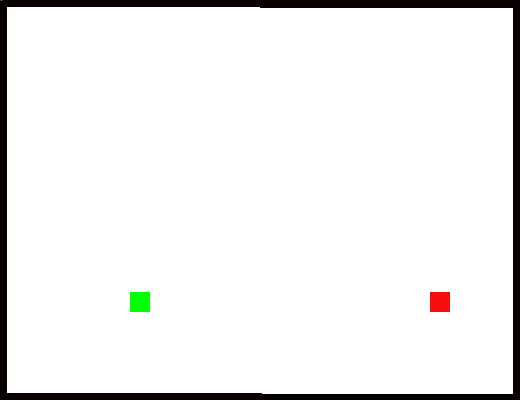
\includegraphics[scale = 0.4]{images/1Dultrasimple.png}
  \caption{View of the simulation of the simple determinist environment}
  \label{fig:my-figure}
\end{figure}

This environment was first developed as deterministic. It was an environment where we knew when and where the target will fire up, and see if the robot was able to learn and take measures against.
It is important to note that we used the agent/algorithm cited earlier : TD($\lambda$), REINFORCE, Random agent and CEM.\\

The next step was to turn the deterministic environment into a random one, to see if the agents were able to adapt.\\

After studying the adaptability of the agents to the simplest environment possible for our task, the goal was to develop an environment where there was not only the action of extinguishing the target, but also moving to it.\\

\begin{figure}
  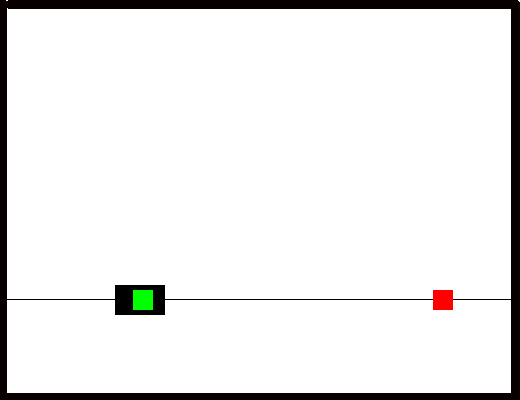
\includegraphics[scale = 0.4]{images/1Dsimple.png}
  \caption{View of the simulation of the 1D environment}
  \label{fig:my-figure}
\end{figure}

The first step was still a deterministic environment, where we knew when and where the targets will light up.\\
The second step was to turn the deterministic environment to a random one.
The final step was to develop the 2D environment. The first 2D-environment developed was a simple one, with only the targets and the robots. It was used to see if the added actions where working accordingly to the real robot.\\

\begin{figure}
  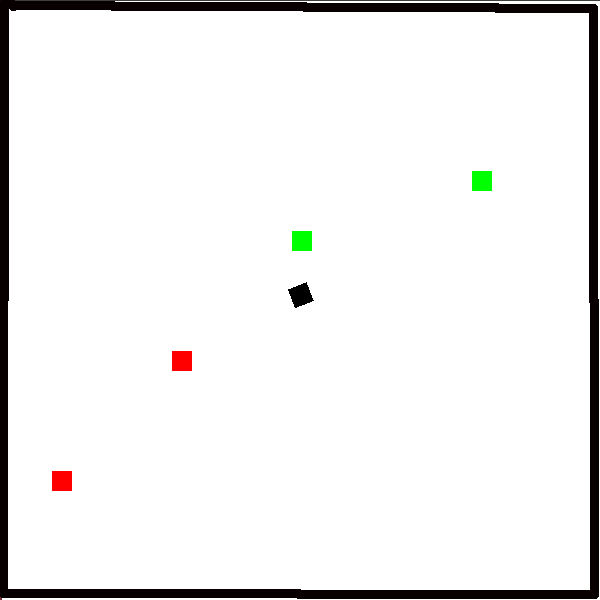
\includegraphics[scale = 0.35]{images/2Dsimple.png}
  \caption{View of the simulation of the 2D environment}
  \label{fig:my-figure}
\end{figure}

Then, we developed a more complex environment to make it as close as possible as reality.\\

\begin{figure}
  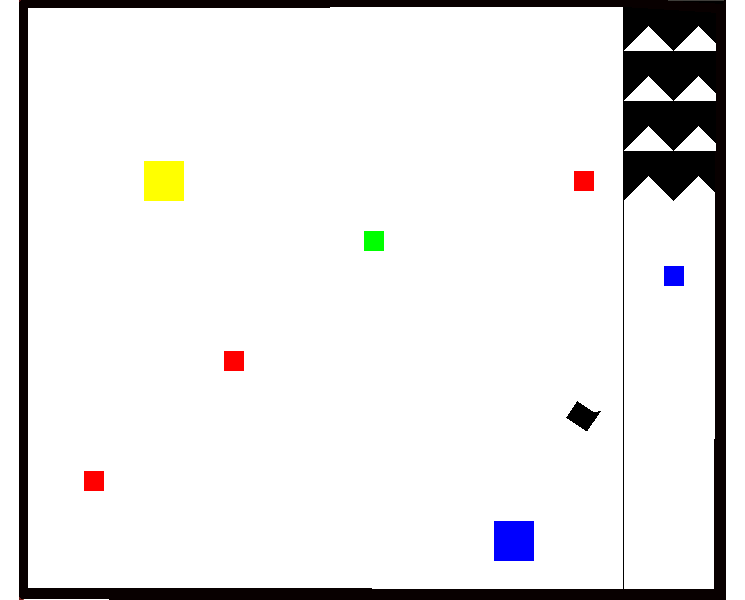
\includegraphics[scale = 0.3]{images/2Dcomplex.png}
  \caption{View of the simulation of the complex 2D environment}
  \label{fig:my-figure}
\end{figure}

To ensure that the environment was close to reality, we discussed the different drawbacks that we needed to implement:
\begin{itemize}
 \item \textbf{the battery} : the energy available for the robot is not infinite, for this, a decrementing counter was implemented, which was decrementing at every action carried out by the robot. There was also a battery zone where the robot could refill up its energy. The battery zone is modeled by the yellow square.\\
 \item \textbf{the robot's water reserve} : as for the battery, the water that the robot can carry is not unlimited. The water was implemented as a counter which was decremented every time the agent used the action to spill water. This water could be refilled in the water zone which was represented as a blue square.\\
 \item \textbf{the refilling water zone} : represented as a blue square, the water refilling zone could see its water level decreasing (which was viewed by the fading blue color) due to water leaks (which are part of the operator actions.). Those leaks are represented by the square in the right side of the window. Each square represent a level of leaks, and the higher the level is, the more water leak.\\ 
 \item \textbf{the human operator} : The operator was designed as a random agent with a fixed random policy.\\
 \item \textbf{the temperature} : The temperature needed also to be modeled, as the robot could not stay to long close to a fire. It was modeled as a counter that was increasing when the robot was in a range from the fire, and decreasing when it was out of this range.\\
 \item \textbf{the fire} : The fires modeled in the environment could be extinguished with only one application of water. We discussed the fact that we needed more than one action to take care of it, but it was not implemented ultimately. But the idea still lies.
\end{itemize}

You can find the environments and videos of the simulations following this address :
\url{https://github.com/TVagneron/Reinforcement-learning}\\

\textbf{Results}\\

In this part, we will display the results of the experiment on the parameters $\lambda$, $\gamma$ and $\epsilon$ which affect the learning update or/and the policy. The following results have been run for a number of 1000 episodes, each episode describing 500 steps. The deterministic environment was tuned to fire one target at a time, every target was lighted up 50 step after the previous one was extinguished.\\




\begin{figure}
\definecolor{ggreen}{rgb}{0.3,0.7,0.4}
\begin{tikzpicture}[scale = 0.7]
\begin{axis}[
grid=major,xmin=1,xmax=1000,ymin=-1,ymax=10,
xtick={0,100,...,1000},
legend entries={$\lambda = 0.02$,$\lambda = 0.1$,$\lambda = 0.01$,$\lambda = 0.5$,$\lambda = 0.005$,$\lambda = 0.8$,legend style={at={(1.52,1.1)}}},
xlabel={Number of episodes},
ylabel={Score},
title={Score growing during learning},width=11cm,height=11cm]
\addplot[color = black, line width=1pt] plot table[x index=0, y index=1]{CSV/Z_origin.csv};
\addplot+[color = blue, line width=1pt] plot table[x index=0, y index=1]{CSV/Z_ralpha01.csv};
\addplot+[color = red, line width=1pt] plot table[x index=0, y index=1]{CSV/Z_ralpha001.csv};
\addplot+[color = orange, line width=1pt] plot table[x index=0, y index=1]{CSV/Z_ralpha05.csv};
\addplot+[color = purple, line width=1pt] plot table[x index=0, y index=1]{CSV/Z_ralpha0005.csv};
\addplot+[color = brown, line width=1pt] plot table[x index=0, y index=1]{CSV/Z_ralpha08.csv};
\end{axis}
\end{tikzpicture}
\caption{Score of the simple deterministic environment for $\lambda$}
\end{figure}

As we can see with fig.6, for a simple environment, changing $\lambda$ does not affect the reward outcome.

%%%%%%%%%%%%%%%%%%%%%%%%%%%%%%%%%%%%%
%\begin{figure}
%\definecolor{ggreen}{rgb}{0.3,0.7,0.4}
%\begin{tikzpicture}[scale = 0.7]
%\begin{axis}[
%grid=major,xmin=1,xmax=1000,ymin=-1,ymax=10,
%xtick={0,100,...,1000},
%legend entries={$\gamma = 1$,$\gamma = 0.5$,$\gamma = 0.7$,$\gamma = 0.3$,legend style={at={(1.52,1.1)}}},
%xlabel={Number of episodes},
%ylabel={Score},
%title={Score growing during learning},width=11cm,height=11cm]
%\addplot[color = black, line width=1pt] plot table[x index=0, y index=1]{CSV/Z_gamma.csv};
%\addplot+[color = blue, line width=1pt] plot table[x index=0, y index=1]{CSV/Z_gamma05.csv};
%\addplot+[color = red, line width=1pt] plot table[x index=0, y index=1]{CSV/Z_gamma07.csv};
%\addplot+[color = orange, line width=1pt] plot table[x index=0, y index=1]{CSV/Z_gamma03.csv};
%\end{axis}
%\end{tikzpicture}
%\caption{Score of the simple deterministic environment for $\gamma$}
%\end{figure}
%%%%%%%%%%%%%%%%%%%%%%%%%%%%%%%%%%%%%%%

\begin{figure}
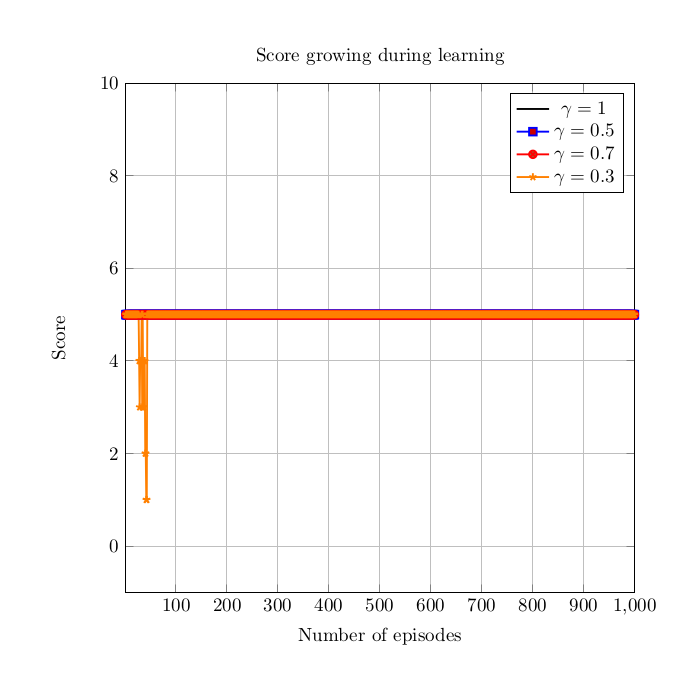
\includegraphics[scale = 0.3]{images/Gamma.png}
\caption{Score of the simple deterministic environment for $\gamma$}
\end{figure}

\begin{figure}
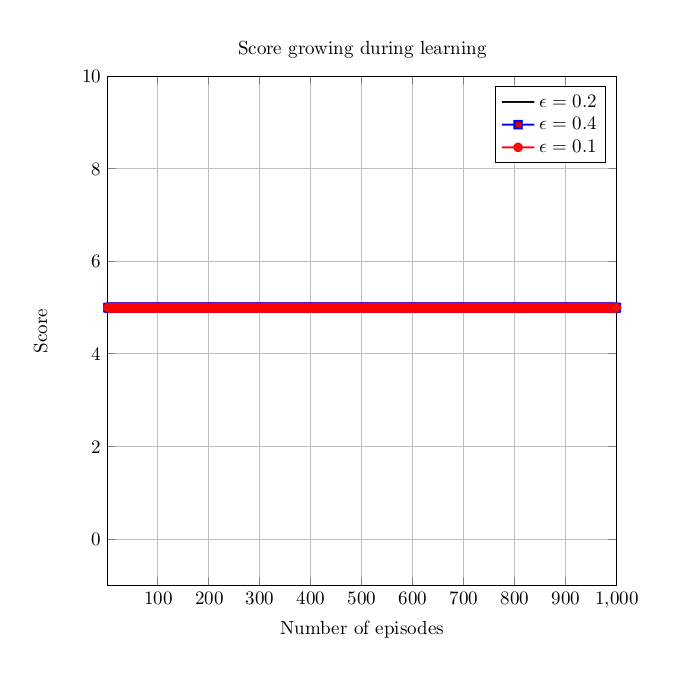
\includegraphics[scale = 0.3]{images/Epsilon.png}
\caption{Score of the simple deterministic environment for $\epsilon$}
\end{figure}

We can observe the same effects for $\gamma$ and $\epsilon$, but what will happen if we complicate the environments? You will see the results for a more complex environment with the figures 9, 10 and 11.

\begin{figure}
\definecolor{ggreen}{rgb}{0.3,0.7,0.4}
\begin{tikzpicture}[scale = 0.7]
\begin{axis}[
grid=major,xmin=1,xmax=1000,ymin=-1,ymax=10,
xtick={0,100,...,1000},
legend entries={$\lambda = 0.02$,$\lambda = 0.1$,$\lambda = 0.01$,$\lambda = 0.5$,$\lambda = 0.005$,$\lambda = 0.8$,legend style={at={(1.52,1.1)}}},
xlabel={Number of episodes},
ylabel={Score},
title={Score growing during learning},width=11cm,height=11cm]
\addplot[color = black, line width=1pt] plot table[x index=0, y index=1]{CSV/origin.csv};
\addplot+[color = blue, line width=1pt] plot table[x index=0, y index=1]{CSV/ralpha_01.csv};
\addplot+[color = red, line width=1pt] plot table[x index=0, y index=1]{CSV/ralpha_001.csv};
\addplot+[color = orange, line width=1pt] plot table[x index=0, y index=1]{CSV/ralpha_05.csv};
\addplot+[color = purple, line width=1pt] plot table[x index=0, y index=1]{CSV/ralpha_0005.csv};
\addplot+[color = brown, line width=1pt] plot table[x index=0, y index=1]{CSV/ralpha_08.csv};
\end{axis}
\end{tikzpicture}
\caption{Score of the deterministic 1D environment for $\lambda$}
\end{figure}


As we can see in the figure, the value of $\lambda$ affects the reward outcome during the learning process. The more the value of the parameter go further from the optimum, the less will be the reward. This was expected as $\lambda$ affects the actuating of the process. We can discuss to what extent $\lambda$ affect the learning process, but it is not the subject of this report, it is to discuss the fine tuning of the parameters in order to optimize the learning process, and thus the policy. The tuning of $\lambda$ can be performed mathematically or experimentally. Here we chose to tune it experimentally. That can be carry out by a machine, which will hasten the process.
We can take note of the spikes that appear at some points during the learning process. Those spikes illustrate the dilemma of prospection/exploitation. This dilemma is the property that the process should not stop to explore, but it should explore less and less.
We can also take note in the difference of reward for a deterministic environment, which is one of the simplest developed here. It brings up the question of fine tuning for the more complex ones, which have more available actions and space.\\

\begin{figure}
\definecolor{ggreen}{rgb}{0.3,0.7,0.4}
\begin{tikzpicture}[scale = 0.7]
\begin{axis}[
grid=major,xmin=1,xmax=1000,ymin=-1,ymax=10,
xtick={0,100,...,1000},
legend entries={$\gamma = 1$,$\gamma = 0.5$,$\gamma = 0.7$,$\gamma = 0.3$,legend style={at={(1.52,1.1)}}},
xlabel={Number of episodes},
ylabel={Score},
title={Score growing during learning},width=11cm,height=11cm]
\addplot[color = black, line width=1pt] plot table[x index=0, y index=1]{CSV/gamma1.csv};
\addplot+[color = blue, line width=1pt] plot table[x index=0, y index=1]{CSV/gamma05.csv};
\addplot+[color = red, line width=1pt] plot table[x index=0, y index=1]{CSV/gamma07.csv};
\addplot+[color = orange, line width=1pt] plot table[x index=0, y index=1]{CSV/gamma03.csv};
\end{axis}
\end{tikzpicture}
\caption{Score of the deterministic 1D environment for $\gamma$}
\end{figure}

 
The addition of $\gamma$ in the learning process also affects the policy (as it appears in both computer codes). We can see, if $\gamma$ is different from one, the reward outcome is zero (fig.10) which is different from the results of fig.7. This could be explained by the complexity of the second environment (with have $\gamma^t$ with a bigger $t$ in fig.10). It was not to be unexpected as $\gamma$ is a parameter that affect the convergence of the sequence.\\

\begin{figure}
\definecolor{ggreen}{rgb}{0.3,0.7,0.4}
\begin{tikzpicture}[scale = 0.7]
\begin{axis}[
grid=major,xmin=1,xmax=1000,ymin=-1,ymax=10,
xtick={0,100,...,1000},
legend entries={$\epsilon = 0.2$,$\epsilon = 0.4$,$\epsilon = 0.1$,legend style={at={(1.52,1.1)}}},
xlabel={Number of episodes},
ylabel={Score},
title={Score growing during learning},width=11cm,height=11cm]
\addplot[color = black, line width=1pt] plot table[x index=0, y index=1]{CSV/origin.csv};
\addplot+[color = blue, line width=1pt] plot table[x index=0, y index=1]{CSV/epsilon4.csv};
\addplot+[color = red, line width=1pt] plot table[x index=0, y index=1]{CSV/epsilon1.csv};
\end{axis}
\end{tikzpicture}
\caption{Score of the deterministic 1D environment for $\epsilon$}
\end{figure}

The variable $\epsilon$ ($1-\epsilon$ is the probability to exploit, and $\epsilon$ the probability to explore) affects the policy: if it is too small, the policy cannot be actualized, resulting in a non-learning behavior, whereas if the value is too high, the policy will be actualized, but to a different policy than the optimum.
 
 As stated previously, those results are only for the deterministic and one dimensional environment. Due to a lack of time, the more complex ones were tested via a random method to verify their functioning. The only tests where we used RL agents were not enough relevant to present them here, but it is important to speak about the optimization of the parameters, and the fact that the development requires to go step by step, as we could let errors slip as we jump over what we could consider as unimportant steps.\\

We also conducted experimentation on the epsilon decay rate, that affects the processing speed, but the tests were not relevant as they brought up an issue that will be stated in the issue part later in the report.\\

We opened a repository on github (\url{https://github.com/TVagneron/Reinforcement-learning}) where you will find all the developed environments, scripts to compile them and a correction to the qfunction script. You will also find the folder containing videos of the experiments.
The first script will compile the chosen environment for running it with the REINFORCE agent. The second script will compile all the environments and allow you to chose the agent with which you can run them.
The qfunction script is a correction of the original qfunction script, where we added print functions to slow down the process (refer to section "Issues" where this issue is developed).\\

\textbf{Issues}\\

Some problems occurred, and this section is here to describe some of them and maybe help to resolve them.

One of the first issue that we encountered when developing our environment was the definition of the observation space, where we needed to define the observations that can be seen by the agent, as for this we defined the states of the targets by a strict binary duo, 0 when the target was extinguished, 1 if it was lighted. To follow strictly our mathematical model, we used a Tuple (that,in openaiGym, are a Cartesian product between a discrete space and a continuous space.) to define the target states, but Tuple where not accepted for observation space, so we needed to define them as a continuous space by the use of arrays and boxes.


The second issue was that when we run our environment, there was an error occurring, stating that the state value was nil. It appears that it was related to a process unable to provide the state at the proper time, resulting in a nil value. This issue was solved by slowing down the process (adding prints to track the error origin solved the problem unexpectedly, but it was also slowed down by adding a wait function in the qfunction). This issue has been observed on two PCs using Ubuntu 14.04. (You can find the issue report following : \url{https://github.com/twitter/torch-twrl/issues/37}).

\section{Conclusion}

This report proposes a short introduction to the possible issues implied by Mixed-Initiative missions.
This kind of missions is prone to grow in the future. 
We studied in this report the use of Reinforcement Learning to develop a policy for the machine tasks.
The simulation environments developed here concern a described firefighter mission involving a human and a robot.
As indicated and illustrated in the experiments it is important to fine tune the different parameters 
as they affect the learning process and the learning speed.
More generally, the domain of machine learning
is a recent domain, so there is a lot more to discover and improve.
Regarding the global Mixed-Initiative missions, 
an other kind of planning algorithm called MOMDP will be used
to infer information about the human operator using the eye-tracker and the electrocardiogram: 
it will allow to improve the interaction between the machine and the human,
and thus the mission achievement.

%\section{First results and future work}

%Equations can be used:
%\begin{equation}
%  \label{eq:tx}
%  s[l] = \sum_{k=0}^{K-1} \sum_{m=0}^{M-1} c_{k,m} g[l-mN] e^{j2\pi \frac{k}{K}l}, \quad l \in \SET{Z}.
%\end{equation}
%Do not forget to define each variable and symbol...

%Figures should be included as floats and properly referenced in the text (Fig. \ref{fig:my-figure}). The same rule applies for tables (Tab. \ref{tab:my-table})

%\begin{figure}[htp]
%  \centering
%  \setlength\figureheight{5cm}
%  \setlength\figurewidth{6cm}
%  % This file was created by matlab2tikz.
% Minimal pgfplots version: 1.3
%
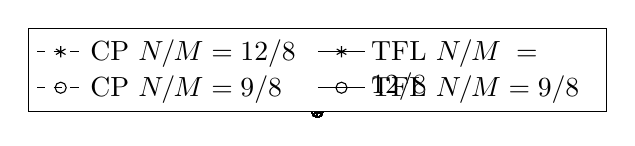
\begin{tikzpicture}

\begin{axis}[%
width=\figurewidth,
height=\figureheight,
at={(0\figurewidth,0\figureheight)},
scale only axis,
separate axis lines,
every outer x axis line/.append style={black},
every x tick label/.append style={font=\color{black}},
xmin=0,
xmax=600,
xlabel={$l_0$},
xmajorgrids,
every outer y axis line/.append style={black},
every y tick label/.append style={font=\color{black}},
ymin=15,
ymax=20,
ylabel={Gain [dB]},
ymajorgrids,
%legend style={legend cell align=left,align=left,draw=black}
legend columns=2,
legend style={text width=8em,legend cell align=left,align=left,draw=black,at={(0.5,1.05)}, anchor=south}
]
\addplot [color=black,dashed,mark=asterisk,mark options={solid}]
  table[row sep=crcr]{%
0	18.2390874094432\\
32	18.2390874094432\\
64	18.2390874094432\\
96	18.2390874094432\\
128	18.2390874094432\\
160	18.2390874094432\\
192	18.2390874094432\\
224	18.2390874094432\\
256	18.2390874094432\\
288	18.2390874094432\\
320	18.2390874094432\\
352	18.2390874094432\\
384	18.2390874094432\\
416	18.2390874094432\\
448	18.2390874094432\\
480	18.2390874094432\\
512	18.2306327719818\\
544	17.9540613758438\\
576	17.6689966399943\\
};
\addlegendentry{CP $N/M=12/8$};

\addplot [color=black,solid,mark=asterisk,mark options={solid}]
  table[row sep=crcr]{%
0	19.9999796047627\\
32	19.9782454264971\\
64	19.9172921503127\\
96	19.819523640774\\
128	19.6869764401989\\
160	19.5221481900787\\
192	19.3264690408576\\
224	19.1028168133025\\
256	18.8524145582619\\
288	18.5769651836831\\
320	18.2797229467138\\
352	17.9588025753321\\
384	17.6198925633198\\
416	17.2597387528296\\
448	16.8807108312221\\
480	16.4832729985219\\
512	16.0669779302672\\
544	15.6289248101717\\
576	15.1692321920288\\
};
\addlegendentry{TFL $N/M=12/8$};

\addplot [color=black,dashed,mark=o,mark options={solid}]
  table[row sep=crcr]{%
0	19.4884747755262\\
32	19.4884747755262\\
64	19.4884747755262\\
96	19.4884747755262\\
128	19.4800794761447\\
160	19.2039363265844\\
192	18.9194155478691\\
224	18.6243664611488\\
256	18.3193439905467\\
288	18.0035198444507\\
320	17.6753775333409\\
352	17.3329477537639\\
384	16.9775142144053\\
416	16.6049465654203\\
448	16.2214034199632\\
480	15.8132879400791\\
512	15.3931020845481\\
544	14.9429381335956\\
576	14.4724841527662\\
};
\addlegendentry{CP $N/M=9/8$};

\addplot [color=black,solid,mark=o,mark options={solid}]
  table[row sep=crcr]{%
0	19.9999188401472\\
32	19.9198402053393\\
64	19.7226565216249\\
96	19.4581952942028\\
128	19.165296513424\\
160	18.8621944283946\\
192	18.5462056497272\\
224	18.2187733804306\\
256	17.8809942229679\\
288	17.5256445475455\\
320	17.1574123511579\\
352	16.769914008492\\
384	16.3698267920046\\
416	15.9497164928657\\
448	15.5024807138218\\
480	15.0375569039195\\
512	14.5394847970002\\
544	14.0174757064722\\
576	13.4597208888491\\
};
\addlegendentry{TFL $N/M=9/8$};

\end{axis}
\end{tikzpicture}%
%  \caption{An accurate caption should be written here}
%  \label{fig:my-figure}
%\end{figure}

%\begin{table}[htp!]
%  \renewcommand{\arraystretch}{1.3}
%  \caption{A detailed caption should be written here}
%  \label{tab:my-table}
%  \centering
%  \begin{tabular}{|c|c|c|c|c|}
%    \hline
%    Filter type & $\sigma_t(\check{\gamma})$ & $\sigma_f(\check{\gamma})$ & $\epsilon_M(\check{\gamma})$ & $\xi(\check{\gamma})$\\
%    \hline
%    RECT & $0.2566N$ & $2.12/M$ & $0.2263$ & $0.1226$\\
%    \hline
%    NR-OBE & $0.2617N$ & $1.44/M$ & $0.1715$ & $0.1874$\\
%    \hline
%    NR-TFL & $0.2580N$ & $0.68/M$ & $0.1839$ & $0.4047$\\
%    \hline
%  \end{tabular}
%\end{table}

% Optional section
\section*{Acknowledgment}

The authors would like to thank Caroline Chanel, because she accepted my participation in this wonderful project.

A huge thank to Nicolas Drougard, for his patience, his support, and all the mishaps we went through.



\bibliographystyle{plain}
\bibliography{references}

\end{document}


